\section{Projektkoordination}
\label{sec:projektkoordination}

Nicht nur die technischen Voraussetzungen, sondern auch die Organisation im Team stellte einen wichtigen Faktor für den Erfolg dar.

%%%%%%
\subsection{Verantwortungsbereiche}
Zunächst analysierten wir genau die uns gegebenen technischen Möglichkeiten, als auch die Aufgabenstellung. Daraufhin verteilten wir Verantwortungsbereiche auf die einzelnen Gruppenmitglieder. Einige dieser Bereiche waren:
\begin{itemize}
	\item Code - Verantwortlich für eine lesbare Struktur und Kommentare im Code
	\item Zeitmanagement - Verantwortlich für Zeitplanung und Einhaltung der Fristen
	\item Dokumentation - Verantwortlich für die schriftliche Dokumentation der Team-Absprachen
	\item Vorträge, LateX und einige mehr
\end{itemize}
Es handelte sich dabei ganz bewusst um Verantwortungsbereiche und nicht um Aufgabenteilung. Idee hierbei war, dass die einzelnen Gebiete nicht ausschließlich von dem jeweils Verantwortlichen beachtet oder ausgeführt wurden, sondern die jeweils Zuständigen darauf achteten, dass alle den entsprechenden Rahmen einhielten. So konnte sich jeder auf seine Verantwortlichkeiten konzentrieren, ohne fürchten zu müssen andere Aspekte zu vergessen. Auf diese Weise war eine gegenseitige Kontrolle und Erinnerung an die Einhaltung der Aufgaben gegeben. Jedes Teammitglied konnte sich stets darauf verlassen, dass eine wichtige Information notiert und an alle Fristen erinnert wurde.


%%%%%%
\subsection{Zeitplan und Meilensteine}
Um einen Zeitplan erstellen zu können, notierten wir zunächst alle extern vom Veranstalter vorgegebenen Ziele mit der entsprechenden Deadline als Meilensteine in unserem Zeitplan. Dazu zählen unter anderem die Endergebnisse und auch die beiden Vorträge. Nachdem wir uns mit der Technik vertraut gemacht hatten, konnten wir auch zu den Meilensteinen Zwischenziele mit der benötigten Zeit und der daraus folgenden Deadline abschätzen. Daraus ergab sich ein Zeitplan, der die gesamte Bearbeitungszeit über Gültigkeit besaß.
\pagebreak
%%%%%%
\subsection{Dokumentation: \textit{Trello}}
Wie bereits erwähnt, legten wir von Anfang an Wert darauf, Absprachen, Entscheidungen aber auch offene Fragen immer schriftlich festzuhalten. Dies sollte natürlich möglichst übersichtlich dargestellt, aber auch stets für alle zugänglich sein. Wir entschieden uns für \textbf{Trello}\footnote[1]{https://trello.com/}. Dies ist ein Online-Organisationsboard, zugänglich über eine Website, womit alle Informationen immer aktuell an einem Ort vorlagen. In Trello können einzelne Listen aus Karten erstellt werden um die Themen zu gliedern. Während Listen die Oberthemen repräsentieren stellen die Karten die Unterpunkte zu den einzelnen Themenbereichen dar.
%%%%%%%%
\begin{figure}[hp] 
  \centering
     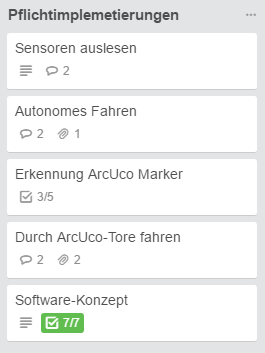
\includegraphics{images/PflichtimplementierungenListe.PNG}
  \caption{Trello-Liste mit Karten}
  \label{fig:Trello-Liste}
\end{figure}
\newline
Dabei werden in der Liste jeweils die Titel der Karten zusammen mit den wichtigsten Informationen angezeigt. So weisen Sprechblasen auf Kommentare und Heftklammern auf Dateianhänge hin. Auch die Anzahl der erledigten Unterpunkte wird angezeigt und bei vollständiger Bearbeitung sogar grün markiert.
\pagebreak \newline
Wählt man nun eine Karte aus, kann man alle weiteren Informationen einsehen. Zuordnungen zu Teilnehmern lassen sich hier realisieren um, zum Beispiel, Aufgabenteilung oder Verantwortlichkeiten aufzuzeigen. Unterpunkte kann man abhaken, was sich in einem Fortschrittsbalken ablesen lässt. Kommentare mit angehängten Dateien lassen sich ebenso realisieren wie Verweise auf Karten aus anderen Listen, um Zusammenhänge darzustellen und schnellen Zugriff zu ermöglichen. Am Ende findet sich unter \textit{"`Aktivität"'} ein Log mit allen Ereignissen dieser Karte zusammen mit dem entsprechenden Zeitstempel.

\begin{figure}[hp] 
  \centering
     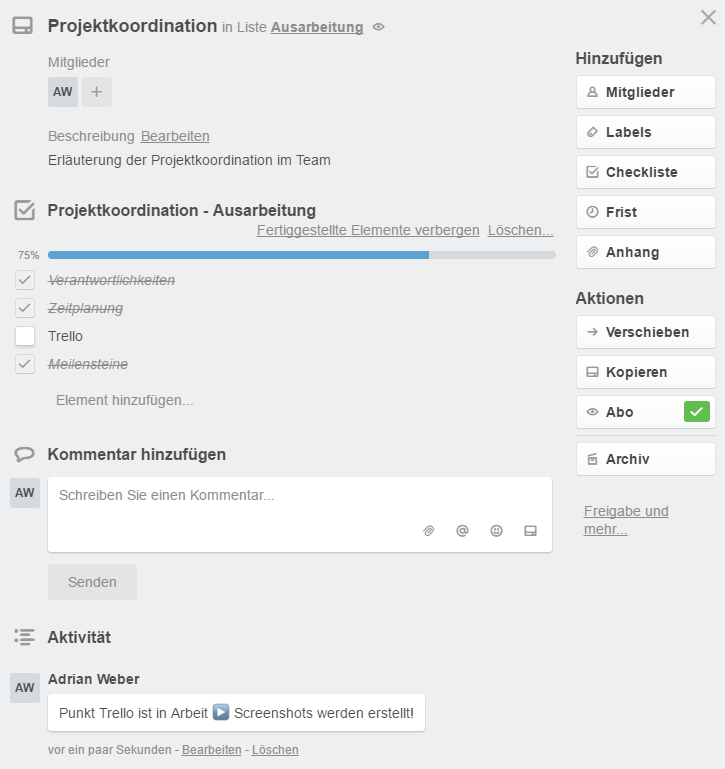
\includegraphics[width=0.9\textwidth]{images/KarteProjektkoordination.PNG}
  \caption{Trello-Karte mit Fortschrittsbalken und weiteren Informationen}
  \label{fig:Trello-Karte mit Fortschrittsbalken, Kommentar und weiteren Informationen}
\end{figure}